\documentclass{article}

\usepackage[utf8]{inputenc}
\usepackage{graphicx}
\usepackage{geometry}   \geometry{margin=1in}
\usepackage{amsmath}

\title{Hot Swappable Pedalboard and Routing System}
\author{Nicholas Pham}
\date{September 2018}

\begin{document}

\maketitle
\begin{center}
    Electrical Engineering \\
    Scott Kuindersma, Jim MacAurthur
\end{center}

\section{Overview}

Many electric guitarists use effect pedals to augment their guitar and amp's sound.  First developed in the 1960s, there are now thousands of pedals available for guitarists to use.  Because of the plethora of options, guitarists need an easy way to compare and interchange effects while still maintaining portability and ease of use.  Current pedalboards and switching systems used to arrange and activate effects have limitations in flexibility.  To solve this, I will develop an integrated, \emph{hot-swappable} guitar effect pedalboard and switching unit which will improve the efficiency and effectiveness with which guitarists use these key pieces of their equipment, allowing players to easily exchange, reorder, and activate their effects.

This project is suitable for my SB specialization because of my interest in guitar effects processors and their control systems.  The work experience I've had, especially at Electro-Harmonix, one of the major players in the guitar industry, has prepared me for this as well.  While at Electro-Harmonix, I worked on a broad similar future product, albeit at a much smaller scale.  I am especially motivated to work on and eventually complete this project because this product will be useful to me as a musician.  In fact, I had already planned on pursuing a similar project on my own time.


\section{Use Cases}

\subsection{Pedalboards}

Guitarist who use multiple pedals often use a \emph{pedalboard} to organize them.  This simplifies transport and setup at rehearsals and performances by leaving the signal and power connections between each pedal intact.  Pedalboards typically consist of some platform structure (the board), a number of effects pedals, and some power supply to power the pedals.  Like all guitar equipment, the signal is connected from one pedal to another via cables with standard 1/4" phone plugs.  Most pedals have one input jack and one output jack, but some stereo pedals can have two of each.  In addition, some pedals accept inputs for external control (often known as expression pedal inputs) which can connect either a direct control voltage, or some foot-actuated potentiometer.  In rarer cases, some more advanced units can accept MIDI connections further control.  Power is typically supplied by a 9VDC, center negative cable, though proprietary supplies also exist.  To actuate a given unit, the guitarist engages one or more footswitches on top of the unit.  To change effect parameters, there are usually one or more potentiometers or switches accessible.

\subsection{Attachment Methods}

Typical pedalboard systems have several issues.  First, the method for attaching individual pedals to the board can sometimes be inconsistent.  The most common method for attachment is via velcro.  This can be an issue for certain pedals, as the adhesive between the velcro surface and the bottom of the pedal can separate, leading the pedal to unintentionally detach from the board.  The velcro can also leave a residue on the pedal, which might reduce its resale value should its owner decide to sell it.  A few benefits of velcro attachment are that pedals can easily be removed and reattached to the board, and that the velcro can be applied to any surface.  In fact, a pedalboard can be constructed from any surface to which the velcro will adhere.  Additionally, the pedals can be placed in any location or orientation on the board, allowing the user to maximize the available surface area.  Another common method is using zip-ties to strap the effects units to the board.  While this technique is unlikely to allow a pedal to inadvertently detach, it does make it very difficult to exchange or reposition pedals because detaching them requires cutting the zip-ties.  Also, the board must have holes in it for the zip-ties to pass through.  From personal experience, this method is also unsatisfactory because the pedals can still shake and move despite being tied down, and the ties can scratch the pedals' paint, again reducing their resale value.

\subsection{Functionality}

Another issue with typical pedalboards is their ease of use.  As each pedal has its own footswitch, any guitarist with more multiple pedals must individually engage each of them.  In live performance, a musician may often want to quickly change their sound, for instance when switching from a rhythm guitar part to a solo.  Because the guitarist must press a number of footswitches to engage the correct set of effects, it can take up to a few seconds for their sound to change, reducing the dramatic effect in the music.  One way this issue has been solved is through the use of \emph{effects-loop switchers}, which can turn on and off effects by dynamically routing signal through or around them.  In this way, multiple effects can be turned on an off via a single command.  However, there are still some issues with this method, as these switchers can take up a significant area on the pedalboard for their enclosure and their cabling, reducing the number of pedals a guitarist can fit on a given board.

\subsection{Flexibility}

Another issue with typical pedalboards is flexibility.  To minimize the physical surface area required for a given number of effects units, pedals on a pedalboard are typically placed as close together as possible such that their footswitches can be individually accessed.  Because the pedals are placed in close proximity, there is often not enough room to unplug the quarter inch phone jacks used for signal connections from the pedals without detaching the unit from the board.  Because of this, A/B comparisons between two effects destined for a single spot on the pedalboard require a significant amount of time to physically swap them.  In addition, the amplifier must be muted to prevent popping that occurs when the cables are disconnected, which could damage the speaker.  The time required for switching between the effects makes it difficult to aurally and viscerally compare the two processors and evaluate their relative merits.  As a result, guitarists may have difficulty deciding between two similar effects, such as two overdrive pedals, and may even be less inclined to switch units because of the difficulty of trying out new ones.  A system that would allow easy switching between pedals would result solve this problem.

\subsection{Users}

This process of choosing different effects units is not only needed when purchasing new pedals.  Guitarists who record in the studio often spend time looking for a distinctive sound that will work with the music they are recording.  Some professional recording guitarists may bring tens of amps and pedals to the studio and use different combinations of processors for each song, or even each track on a song.  Because of the issues described above when comparing different effects, the studio guitarist must spend precious studio time deciding on their equipment, instead of focusing on their performance.  With high recording studio time costs, a faster system of switching between effects will save musicians and record labels time and money in producing records.

An additional application for such a quick switching system is for performing guitarists who fulfill different roles at different times.  A guitarist who plays in multiple groups of different styles may want to use a different set of effects units for each gig; for example, they may use a heavy \emph{distortion} and a \emph{delay} when playing in a rock band, but instead need a \emph{compressor} and an \emph{auto-wah} for a funk group.  The performing musician might also want to use one of the aforementioned automatic switching systems to set up \emph{presets}, or combinations of certain effects that are turned engaged at once to avoid needing to manual turn on each pedal.  To reduce the amount of equipment to transport, it is ideal to bring only the effects pedals needed for each gig, but automatic switching systems routinely sell for the price of several effects units, so few guitarists would purchase more than one.  An easily swappable pedalboard integrated with an automated switching system would be ideal for performing musicians.


\section{Previous Work}

\subsection{Typical Methods}
The most ubiquitous velcro style pedalboard is the Pedaltrain brand \cite{CHANDLER:2000}\cite{PEDALTRAINSITE}.  Zip-tie style pedalboards include the Holeyboard from Chemistry Design Werks \cite{TRIFILIO:2017}\cite{HOLEYBOARDSITE}.

\subsection{Magnetic Attachment}

A more interesting attachment method are magnets, which I also plan to use in my design.  The Earthboard from Rare Earth Music LLC uses magnets to attach pedals to the board.  This is accomplished by first attaching the pedals to a base plate via velcro, then using magnets on the plate, the pedal is attached to the board.  One great feature of this board is that power is delivered to the pedals through the plate.  As the plates are mounted to two rails, the pedalboard's power supply places a voltage across the rails, which is connected to the pedal proper via a cable attached to the plate.  Thus, when removing pedals, the user must only disconnect the input and output signals before removing the plate \cite{EARTHBOARDSITE}.

I plan to begin with this magnetic attachment method, using plates to interface between pedals and the pedalboard.  However, this particular product fails to take full advantage of the modular ability of such a design.  The signal connections are not integrated with the detachability, and the pedal is still attached with velcro to the plates, leading to the same issues of detachment and residue experienced by the velcro method.

\subsection{Bracket Attachment}

U.S. Patent Grant US9620094B2 describes an improved method for attaching pedals to a pedalboard \cite{ABBATE:2016}.  Using small brackets which are directly mounted to the pedal enclosure via the bottom cover screws, this method for mounting pedals is much more stable and solid than velcro or zip-tie methods, while also using few external materials.  However, this implementation describes directly attaching the pedals to the pedalboard, which will require other screws.  This means the pedal placement will be fairly permanent and it will be difficult to swap out pedals, necessitating the use of external tools such as a screwdriver.  I propose to use a similar technique to mount the pedals to the bottom plates as will be described in section \ref{Approach}.

\subsection{Modular Effect System}

U.S. Patent US4479238A describes an effect system incorporating a main parent enclosure which contains power and signal routing circuits and receiving slots for effect modules \cite{SPECTOR:1982}.  These modules contain effects circuits built into a special form factor that allows them to be inserted into the slots and make signal and power connections with the main unit.  The main enclosure contains routing circuits which can choose, remotely or on the front panel, which effects should be connected, much like the automatic routing systems described previously.  In addition, the housing automatically bypasses any slot in which no module is fully inserted, preventing issues with "hot-swapping", or removing the effect card while the system is in use.

This system does a nice job of allowing different combinations of effects to be tested, but it does have a significant limitation.  The effect modules must be of the correct card format, which limits the user to specifically designed units.  As the guitar pedal form factor is so ubiquitous (though not exactly standardized: pedals may come in many shapes and sizes), a guitarist using this system would not be able to incorporate the majority of effects units offered today, and would not be able to use any pedals they already own.  In addition, because of their design, these card modules cannot be used in absence of the main enclosure unlike normal guitar pedals, further limiting their flexibility.  I will likely take inspiration from the switching and hot-swappable capabilities of this invention in my design. 

\section{Approach} \label{Approach}

My approach to solving this problem involves something of a synthesis of the above prior art.  Each individual invention solves some part of the main issue, but many of their workings must be combined in order to be truly effective.

In summary, the hot-swappable guitar effects pedalboard and routing system will use standardized plates to interface between the pedals and the switching system.  The plates will have signal, control, and power connections to the pedal.  The plates will also include mechanical locating features and ferromagnetic materials which will attach to corresponding receiving features on the pedalboard itself.  By a system of exposed electrodes, the plates and pedalboard will be able to interface signal, control, and power between them.  The receiving locations in the pedalboard will also include some method by which to detect when a plate is not inserted, which will be used to prevent damage to other equipment by bypassing the connections to the plate.  Finally, the pedalboard will contain a system to automatically route signal and controls to different plates based upon input from some control device, such as a foot-operated MIDI controller.

\subsection{Pedal-Plate Mounting}

The pedals will mount directly to the plates via holes in the plates, through which the pedals' bottom cover screws will pass.  The plates will act something like a secondary bottom cover (see Figure \ref{fig:plate_pedal_mounting}).

\begin{figure}
    \centering
    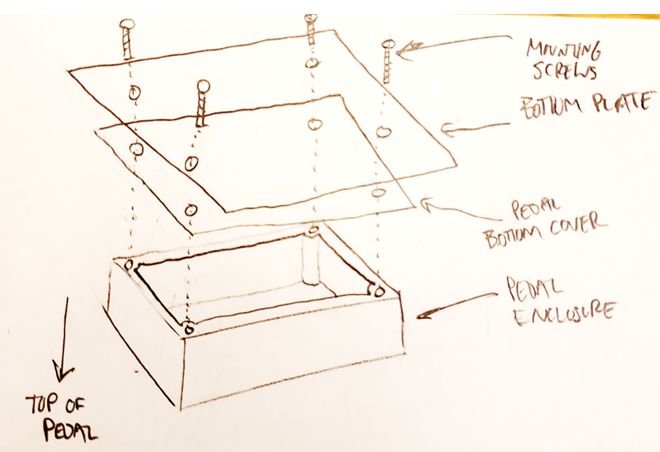
\includegraphics[width = 0.6 \textwidth]{plate_pedal_mounting_img}
    \caption{Assembly of bottom plate to pedal.  Note that the pedal is face down.  The pedal's bottom cover is in contact with the rest of the pedal's enclosure, then the bottom plate rests on the bottom cover.  The pedal's mounting screws are inserted through holes in the bottom plate and cover into the enclosure.}
    \label{fig:plate_pedal_mounting}
\end{figure}

This is an improvement over the Earthboard's method, as the pedals are directly fixed to the plates, as opposed to still being velcroed.  This connection will stay stable and firm, and is also aesthetically pleasing, as no there will be no visible attachment devices or residue.

One issue with this approach is that pedal enclosure sizes are not standardized across all manufacturers, so holes of different locations will need to be included.  It might be useful for the plate to be easily modified by the user so that non-standard mounting locations may be used.

\subsection{Pedal-Plate Electrical Connections}

Like the Earthboard, the plate will make electrical connections to the pedal by means of cables.  This allows pedals of any shape and orientation to be connected into the system.  However, unlike the Earthboard, the plates will connect both power and signal to the pedals, allowing the entire plate and pedal to be removed from the pedalboard without having unplug any standard jacks.

\subsection{Plate-Pedalboard Interface}

The crux of this project is the interface between the plates and the pedalboard receptacles.  As with the Earthboard, this device will use magnets to attach the plates to the pedalboard.  However, instead of the magnets being located on each plate, they will instead be located in the receptacle.  Assuming that the user has more pedals/plates than the pedalboard has room for, this will reduce the cost of the system as each pedal-plate need only be made of some ferromagnetic material, rather than contain potentially expensive magnets.

To make electrical connections between the plate and the pedalboard, a set of electrodes will be left exposed on the plate.  When the plate is inserted, these will make mechanical and electrical connections with spring loaded \emph{pogo-pins} on the pedalboard.  See Figure \ref{fig:plate_board_interface}.

\begin{figure}
    \centering
    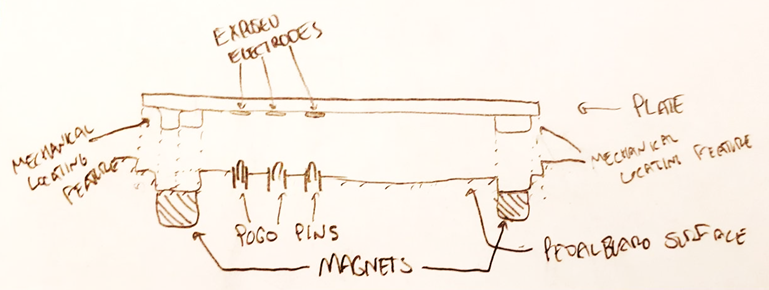
\includegraphics[width =  \textwidth]{plate_pedalboard_interface_img}
    \caption{Side view.  Note the locating features from the plates mirrored on the pedalboard.  These align the pogo-pins and exposed pads, allowing for a secure and consistent connection every time.}
    \label{fig:plate_board_interface}
\end{figure}

To ensure that the correct pogo-pin always connects to its corresponding electrode, the locating features must only fit correctly in one orientation; a symmetrical design would not work.  See Figure \ref{fig:plate_bottom}.

\begin{figure}
    \centering
    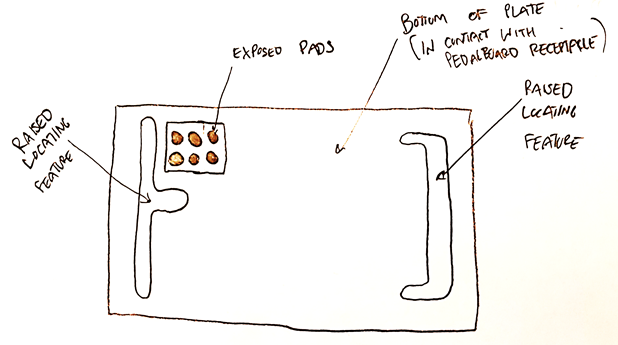
\includegraphics[width = 0.6 \textwidth]{plate_bottom_img}
    \caption{Bottom view of pedal plate.  This side will be in contact with the pedalboard underneath.  Note the asymmetrical locating features and the exposed electrodes.  Though in most cases only four electrodes are needed (input, output, power, and ground), in some cases such as effects with stereo inputs and outputs, up to six electrodes may be useful.}
    \label{fig:plate_bottom}
\end{figure}

In addition to the features described thus far, the receptacle must have some sensor to determine when a pedal plate is about to be removed so the integrated switching system can bypass it.  This may require some experimentation, but one simple design would involve an additional pogo-pin and electrode that loses before the others do (perhaps the pogo-pin is recessed further into the chassis of the pedalboard).  This would give some time for the plate signal path to be bypassed before the signal and power electrodes lose contact.

\subsection{Switching System}

To be fully useful to the studio and live performer, the switching system should allow for any of the effects to be combined in any order or routing configuration.  This includes parallel combinations in addition to the standard series connections typical of most guitar pedalboards, which gives guitarists access to additional tonal options.  In addition, the switching system should be able to change the routing in real time, with no perceptible interruption to the user.

One method of doing this may be using a crosspoint switch, such as the MT8808 from Microsemi \cite{Zarlink:MT8808}.  This chip has:

\begin{itemize}
    \item -95dB OFF feed-thru on its switches, so it can reliably be used to control the signal
    \item 45 MHz bandwidth which should have no problem passing audio signals
    \item 0.01\% THD which is adequate for such a switching system
    \item 20 nS minimum data-hold time for switch data
    \item 100 nS maximum time delay between switch enable and the switch status changing
\end{itemize}

The last two specs suggest that a worst case switching time would be about 

\begin{equation}
    8^2 \text{switches} * 20 \text{nS per switch} + 100 \text{nS delay} = 1.38 \text{mS}
\end{equation}

which should not be perceptible, though the minimum perceptible switch time should be experimentally determined and correlated with existing research.

\subsection{Specifications and Unknowns}

Most of the specifications of the unit are related to signal quality and switching speed, but the first demonstrates success in solving the real issue.

\begin{itemize}
    \item Decrease time required to swap out a pedal by a factor of 5
    \item Signal Attenuation/Degradation < -0.5dB, 20-20kHz through all switches
    \item Tentatively: Noise floor -80 dB (see below for more details)
    \item Switching time not noticeable ( < 10 mS ?)
    \item Switching noise under noise floor
\end{itemize}

Unlike most pieces of guitar equipment, this type of unit is designed to pass signal with high fidelity as opposed to obviously effecting it in some way.  Thus, these specifications must be at least as good as the other components in the system.  For example, the noise floor of the switching system need not be -100 dB if the noise floor of typical guitar amplifiers is only -70 dB.  Similarly, if a guitarist or listener can only detect 10 mS disruptions to the sound, the unit does not need to switch faster than this.  Thus, a number of experiments must be performed in order to determine the exact specifications required, including:

\begin{itemize}
    \item
        Measure time required to remove and replace single pedal from pedalboard setup, using different methods of pedal attachment described above.
    \item
        Measure typical noise floor for guitar equipment.
        \begin{itemize}
            \item Guitar (both Humbucker and Single-Coil)
            \item Pedals (range of distortion levels)
            \item Amplifiers (range of distortion levels)
        \end{itemize}
        The combination with the lowest noise floor should give starting point for this unit's specification.
    \item
        Measure human perception of switching time to determine required switching speed
    \item
        Measure human perception of signal degradation 
\end{itemize}

In addition to these considerations, there are some others that will need to be sorted out:

\begin{itemize}
    \item 
        Some guitarists value mechanical switching for a "purer" sound as compared to solid-state switching.  In fact, some high end switching units use mechanical relays instead of solid-state switches to cater to this demand.  I will perform a test to compare the signal degradation and frequency response of solid-state switches such as those in the MT8808 with relay switches to determine if there is indeed any merit to this preference.
    \item
        Because the pedalboard will have receptacles for the pedal plates, the board will only be able to support a finite number of plates and therefore pedals at once.  Finding the right number is important, as this will have an impact on the product's real and perceived usefulness.  If there are too many slots, then the easy hot-swappability feature is less important, as all of the pedals could be left on the pedalboard or connected to an automated switching system.  On the other hand, if there are too few slots, there may not be enough tonal options available to the player.  My gut instinct is that six slots is a reasonable starting point, but more thought must be given to this.
    \item
        As pedal plates are switched in and out for different performances, it would be helpful to reflect this on the switching system's user interface.  In addition, the user may want the switching system's settings to update based on which pedals are connected (they may want a different set of presets available with Pedal X vs Pedal Y).  One way of doing this would be to include a small programmable memory with each pedal plate and storing key information about the pedal, such as a unique identifier and its power supply voltage, which could inform the switching system to act appropriately.  However, this would add complexity and may not be necessary.
        
    \item
        In some cases, it may be useful for the switching system to automatically prevent feedback loops, such as when the user attempts to connect the output of a pedal to its input.  However, feedback could be used for musical effect in some circumstances, such as recordings, so this feature might be one that can be disabled by the user.
        
    \item
        I will need to determine a proper pull strength of the magnets that is a good compromise between the plates not falling off and it being too difficult to remove a plate with one hand.  I should be able to get some advice on this to get in the ballpark.
\end{itemize}

\section{Related Courses and Skills}

\subsection{Experience}

This project will rely heavily on analog and digital circuit design skills developed in ES-52 and ES-154.  Programming skills from CS-50 and CS-61 will be helpful in working on the embedded system to control the switching and automatic bypassing when no plate is inserted.  Some of the mechanical engineering techniques I learned including CAD modeling and machining will be helpful in bringing the entire system together.

In addition to material covered in the classroom, I have picked up many useful skills through some of the internships I have worked, namely at Electro-Harmonix and Bose.  At these companies, I learned to use CAD tools for schematic entry and PCB layout, which will be necessary for designing the circuitry.  In both positions, I worked with a small team on a new product from concept to prototype, and exposure to this process will aid me on this project.

\subsection{Resources}

I anticipate needing the aid of the Active Learning Lab staff to offer guidance, especially on the mechanical design of this project.  I will also need access to their equipment when I fabricate prototypes.

I will need access to schematic entry and PCB layout CAD software to design the circuits.  I have experience with Cadence Allegro though I prefer Altium Designer.  When physically assembling the circuits, I will likely need to use an external service to manufacture the boards, which I should be able to populate manually.

In addition to these, it would be beneficial to have access to a variety of guitar pedals to perform some of the experiments listed above.

\section{Schedule}

Below is a rough schedule for the next few months.  As I am sure my plans will change as this moves forwards, I don't feel that it is worth more detailed scheduling now.  In particular, further weeks are more vague and general, as their specific tasks will evolve based on what has been completed.  In particular, the iteration stages are highly dependent on how well my prototypes meet the desired specifications.  Despite this imprecision, making this schedule has proved useful in giving me an idea of how much time I really have.


\begin{table}[h!]
\begin{tabular}{llp{4in}}
Weeks    & Dates         & Plan \\
\hline
1 \& 2   & 9/2 - 9/15    &  Complete and revise Project Proposal and meet with advisers      \\
3 \& 4   & 9/16 - 9/29   &  Conduct experiments described above to help refine specifications.  Begin higher level block diagrams of system.  Progress Report \#1 due 9/28    \\
5 \& 6   & 9/30 - 10/13  &  Begin prototyping key features, such as pedalboard - plate interface.  Develop lower level block diagrams and begin schematic design.    \\
7 \& 8   & 10/14 - 10/27 &  Schematic entry and PCB design.  Begin mechanical CAD modelling.    \\
9 \& 10  & 10/28 - 11/10 &  Review electrical design, send out for fabrication.  Begin writing firmware for embedded system.  Progress Report \#2 due 11/5    \\
11 \& 12 & 11/11 - 11/24 &  Fabricate mechanical parts.  Assemble circuit boards.  Perform preliminary testing and begin iterating.    \\
13 \& 14 & 11/25 - 12/8  &  Finish assembling prototype, continue testing     \\
15 \& 16 & 12/9 - 12/22  &  Summarize testing and outline goals/changes for next iteration.  Oral Design Review/Presentation 12/10    \\
17 \& 18 & 12/23 - 1/5   &  Winter Break: expect little progress    \\
19 \& 20 & 1/6 - 1/19    &  Continue firmware (may be done off-campus)    \\
21 \& 22 & 1/20 - 2/2    &  Complete firmware, iterate design if specifications are not met   \\
23 \& 24 & 2/3 - 2/16    &  Fabricate/Assemble iterated design and analyze.  Progress Report \#3 due 2/15    \\
25 \& 26 & 2/17 - 3/2    &  Analyze iterated design.    \\
27 \& 28 & 3/3 - 3/16    &  Implement reach features if time permits, else continue iterating and analyzing.  Begin outlines for Final Report.  Progress Report \#4 due 3/5   \\
28 \& 29 & 3/17 - 3/30   &  Prepare for presentation.  Write final report, make last minute changes.  Final Oral Presentation 3/25  \\
30 \& 31 & 3/31 - 4/13   &  Revise final report.  Final Written Report due 4/5    
\end{tabular}
\end{table}

\section{Budget}

Like the schedule, the budget is also vague right now.  The number of iterations I have will certainly affect the cost.  However, as I plan to use readily available parts and perform most of the mechanical assembly myself, the cost should not be too significant.

Something I would like to look into is temporarily obtaining a number of guitar effects pedals to use for testing (SNR, mechanical design, etc...).  It might also be useful to have these for demonstrations and testing of my prototypes and final product throughout the year.

Note that electronics components are available from Mouser.

\begin{table}[h!]
\begin{tabular}{llll}
Item                     & Quantiy & Unit Cost & Total      \\
\hline
2 layer PCB from PCBgogo                    &         &           & $\sim$\$60 ?    \\
Phone Connectors Mono Male (CUI)            & $\sim$18     & \$3.50    & $\sim$\$60 \\
NRJ6HM1 Phone Connectors Female (Neutrik)   & $\sim$6      & \$0.60    & $\sim$\$4  \\
MT8808 Analog/Digital Crosspoint SW 8x8     & 1       & \$10      & \$10            \\
Misc Electronic Components                  &         &           & \$30 ?          \\
Microcontroller                             & 1       & $\sim$\$5 & \$5             \\
4 lbs pull neodymium magnets, McMaster      & 2 x 6   & \$5       & \$60            \\
Misc mechanical components, materials       &         &           & \$100           \\
\textbf{Total}                              &         &           &  $\sim$\$350    \\
\end{tabular}
\end{table}

\newpage
\bibliography{ThesisSources}
\bibliographystyle{plain}


\end{document}
